 \begin{figure}[H]
     \centering
     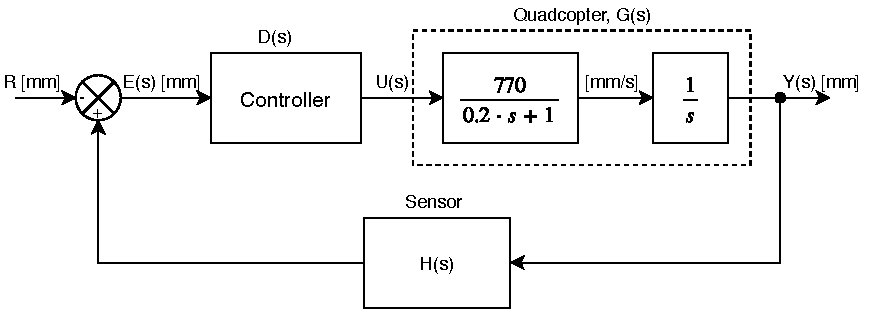
\includegraphics[width=\textwidth]{figures/ch_design/controller/ControlDiagramTF.pdf}
     \caption{Block diagram illustration of the control system  to control the levitation of the Quadcopter.}
     \label{fig:controlDiagram}
 \end{figure}

%To avoid steady state error, it is necessary to examine PID controller, which stands for proportional integrate derivative controller.
To make the full control loop, there are needed two more components apart from the transfer function. This can be seen in figure \ref{fig:controlDiagram}. From this figure it is visual that there is needed a function for the sensors and a controller of the control loop. 
First the function for the sensor will be found and afterward the PID controller will be examined with all the components.


\section{Feedback control loop}\label{s:feedback_loop}
To design a control system, a feedback control loop is needed. Normally it will just be a factor like 1, but in this situation, the feedback in the control loop, will be the feedback from the distance sensors. To get an expression for the feedback, a equation is used. Because the feedback is coming from a sensor, that need to sample the data needed to the feedback, the expression in equation \ref{eq:formular_sampling_feedback} is used \cite{digital_control}.
\begin{equation}\label{eq:formular_sampling_feedback}
    H(s)=\frac{2/T}{s+2/T}
\end{equation}
In this equation the T is the sampling time for the sensor, in this case the sampling time is $25\ ms$, so the expression for the feedback loop will be as seen in equation \ref{eq:feedback_loop}\cite{feedback_control}.
\begin{equation}\label{eq:feedback_loop}
    H(s)=\frac{\frac{2}{0.0025}}{s+\frac{2}{0.0025}}
\end{equation}

\section{PID controller}
To figure out what kind of controller there are needed in the system, to get the right output of the system. In this case the PID controller of a first order close loop system will be explained to find the best suited controller for the system. In the PID controller, there are both a proportional part, an integral part and a derivative part. All these three parts have influence on the output signal. 

\begin{figure}[H]
    \centering
    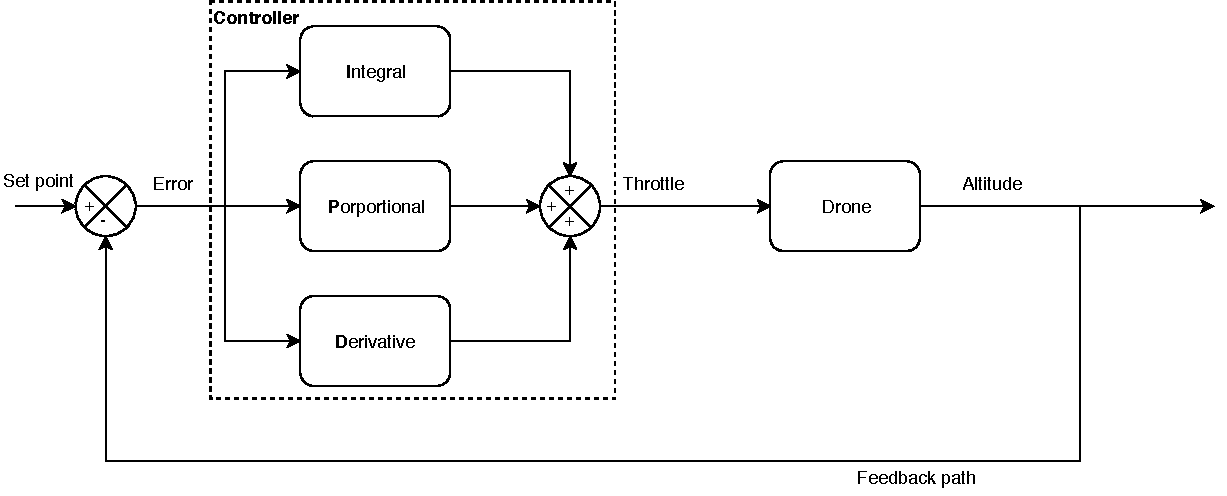
\includegraphics[width=0.9\textwidth]{figures/ch_design/PIDController/PIDControl.pdf}
    \caption{Illustration of a PID controller connected in a control loop.}
    \label{fig:PID_Controller}
\end{figure}
As shown in figure \ref{fig:PID_Controller} the focus for this control system, will be on a closed loop control system. This is used because of the implementation of the sensors in the system. To control this system a PID controller will be used, or a part of it. First the different parts of the PID controller will be explained. The three parts that will be explained are the proportional part, the integral part and the derivative part \cite{digital_control}.

\subsection*{Proportional controller}
The proportional control is in most cases the main driving force in a controller. The proportional control changes its output in proportional to the error. 
The function for the proportional correction, is shown in equation \ref{eq:kp}.
\begin{equation}\label{eq:kp}
    \frac{U(s)}{E(s)}=K_p
\end{equation}
In equation \ref{eq:kp}, the E(s) function is the error on the input and U(s) is the output after the controller part as seen on figure \ref{fig:controlDiagram}.
If the $K_p$ gets increased, a larger error can be corrected, but in situations the $K_p$ value gets too big, the error will get larger too. The proportional controller can only correct constant error on the gain. By choosing a very small $K_p$ value the error is big, and by choosing $K_p=1$ there will be corrected no error. If a too big $K_p$ value is chosen will the control loop begin to oscillate and eventually become unstable. If the $K_p$ is too low, the control loop will not respond enough to disturbances or set point changes. The proportional controller is used for set the phase margin and gain margin to the optimal setting \cite{digital_control}. 


\begin{comment}


The following graph \ref{fig:P_Control} will illustrate a proportional control, and what will happen, when a drone rises to a giving altitude, which in this case it will be 40 cm. 
\begin{figure}[H]
    \centering
    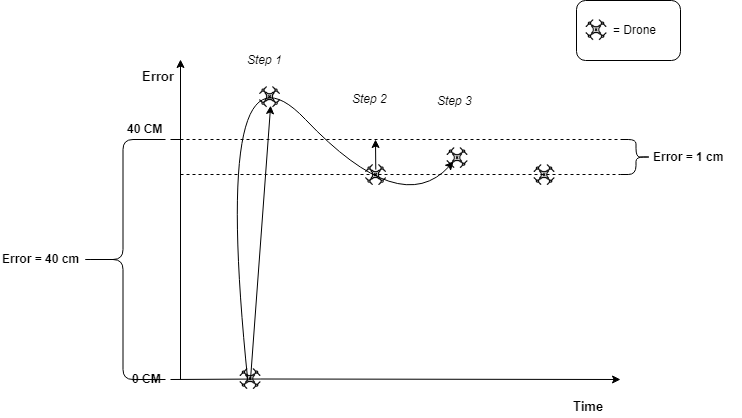
\includegraphics[width=0.8\textwidth]{figures/ch_design/PIDController/ProportionalGraph.png}
    \caption{Illustration of a proportion control system.}
    \label{fig:P_Control}
    \end{figure}
The graph \ref{fig:P_Control} at the starting point there is an error of 40 cm, since there is large of error, it will generate a large propeller speed, which the drone will rise. In step 1 at 40 cm, the error is equal 0, and at this point the propeller speed decrease and the drone will fall back to earth. However, since the propeller speed is large, it will have overshoot as seen in the graph (step 1). When it is under 40 cm the propeller speed will increase again and since the error is 1 and is not large, it will increase the propeller speed slightly as seen at graph (step 2). To hover the drone, its need a certain propeller speed, where the lifting force is exactly equal to the weight of the drone, that speed will hover the drone.    

To hover the drone at certain altitude will depend on the controller gain and propellers speed. In this example we assume that at 80 rpm the drone will hover, if the proportional gain is 2 and the drone is at starting point, which the error is 40 cm, the drone would hover right at the ground level since 2 \(\times\) 40 is 80 rpm. The following graph \ref{gra:P_Control_graph} illustrates where the drone will hover, when the gain increases.

\begin{figure}[H]
    \centering
    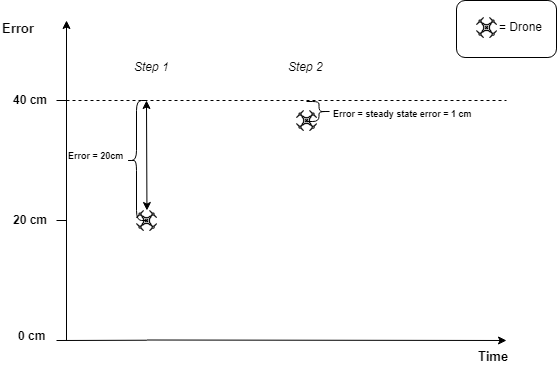
\includegraphics[width=0.6\textwidth]{figures/ch_design/PIDController/ProportionalGraph1.png}
    \caption{Proportional control graph.}
    \label{gra:P_Control_graph}
    \end{figure}
The graph \ref{gra:P_Control_graph} at step one the proportional gain is set to 4, which the error is reduced to 20 cm, since the drone is closer to the set point. In step two the proportional gain is 80 and the drone is hovering at 39 cm, which the error is 1 cm. This constant error is also called steady state error and this will never be eliminated in proportional control. There is a need of a or control mode, which can use past information to eliminate the steady state error. 

\end{comment}

\subsection*{Integral controller}
Apart from the proportional controller, an integral controller always works on the changing error, to make the error goes to zero. The ways this controller works on is by continuously increment and decrements the controller's output to reduce the error from the loop. 

The error correcting time can depend on the sixe of the error. The time used is defined be the size of $T_I$ in the equation, can also be seen in equation \ref{eq:integral_control} \cite{digital_control}. 

\begin{equation}\label{eq:integral_control}
    \frac{U(s)}{E(s)}=\frac{k_I}{s} \to u(t)=k_I \int_{t_0}^t e(\tau) \ d\tau
\end{equation}
In this equation $k_I$ is th integral constant. It can be seen from the equation, that the size of $k_I$ has influence on the reaction time. If this value is small the reaction time will be fast, but if it is a big value it will have the opposite effection. If the time is set to small the control part can be slow, but if the time is set to big the control loop can begin to oscillate and become unstable. The upside of using a integral controller, is to add more gain for the transfer function. By doing this the steady-state behavior will be improved along side the adding of gain. 
If the $k_I$ get to big it can also increase the overshoot for the control loop\cite{digital_control}. 


\subsection*{Derivative controller}
The derivative controller is mostly used in a motion controller. There are some problem related to this type of controller, it is very sensitive to measurement noise and it makes it difficult to make trial-and-error tuning.  It still make the response faster then by using a PI-controller only \cite{digital_control}. 

The way the derivative controller works is by producing the output on the rate of changes of the errors. By doing this the derivative control, can be said to work on the errors, by correcting them by look on the past. This means the controller correct errors at a high rate, and if there are no errors the derivative controller will be zero. The equation for the derivation controller can be seen in equation \ref{eq:derivative_control} \cite{digital_control}.

\begin{equation}\label{eq:derivative_control}
\frac{U(s)}{E(s)}=k_D \cdot s
\end{equation}

In this equation the $k_D$ is the derivative time. The larger the derivative time is set to, the more higher the action form the controller will be, but if the time is set to high the controller will begin to oscillate and become unstable. And if the derivative time is to small the influence on the output will be slower \cite{digital_control}. By implementing a derivative controller, increase the phase. By increasing the phase, the phase margin also improves and thereby the damping of the transfer function.

\section{Differences between the PID-controllers parts}\label{s:different_pid}
To compare the different combination between the PID-controller's parts, first a bode plot of all the components will be made to compare how they infect the bode plot. This bode plot can be seen figure \ref{fig:PID_bode}.

\begin{figure}[H]
    \centering
    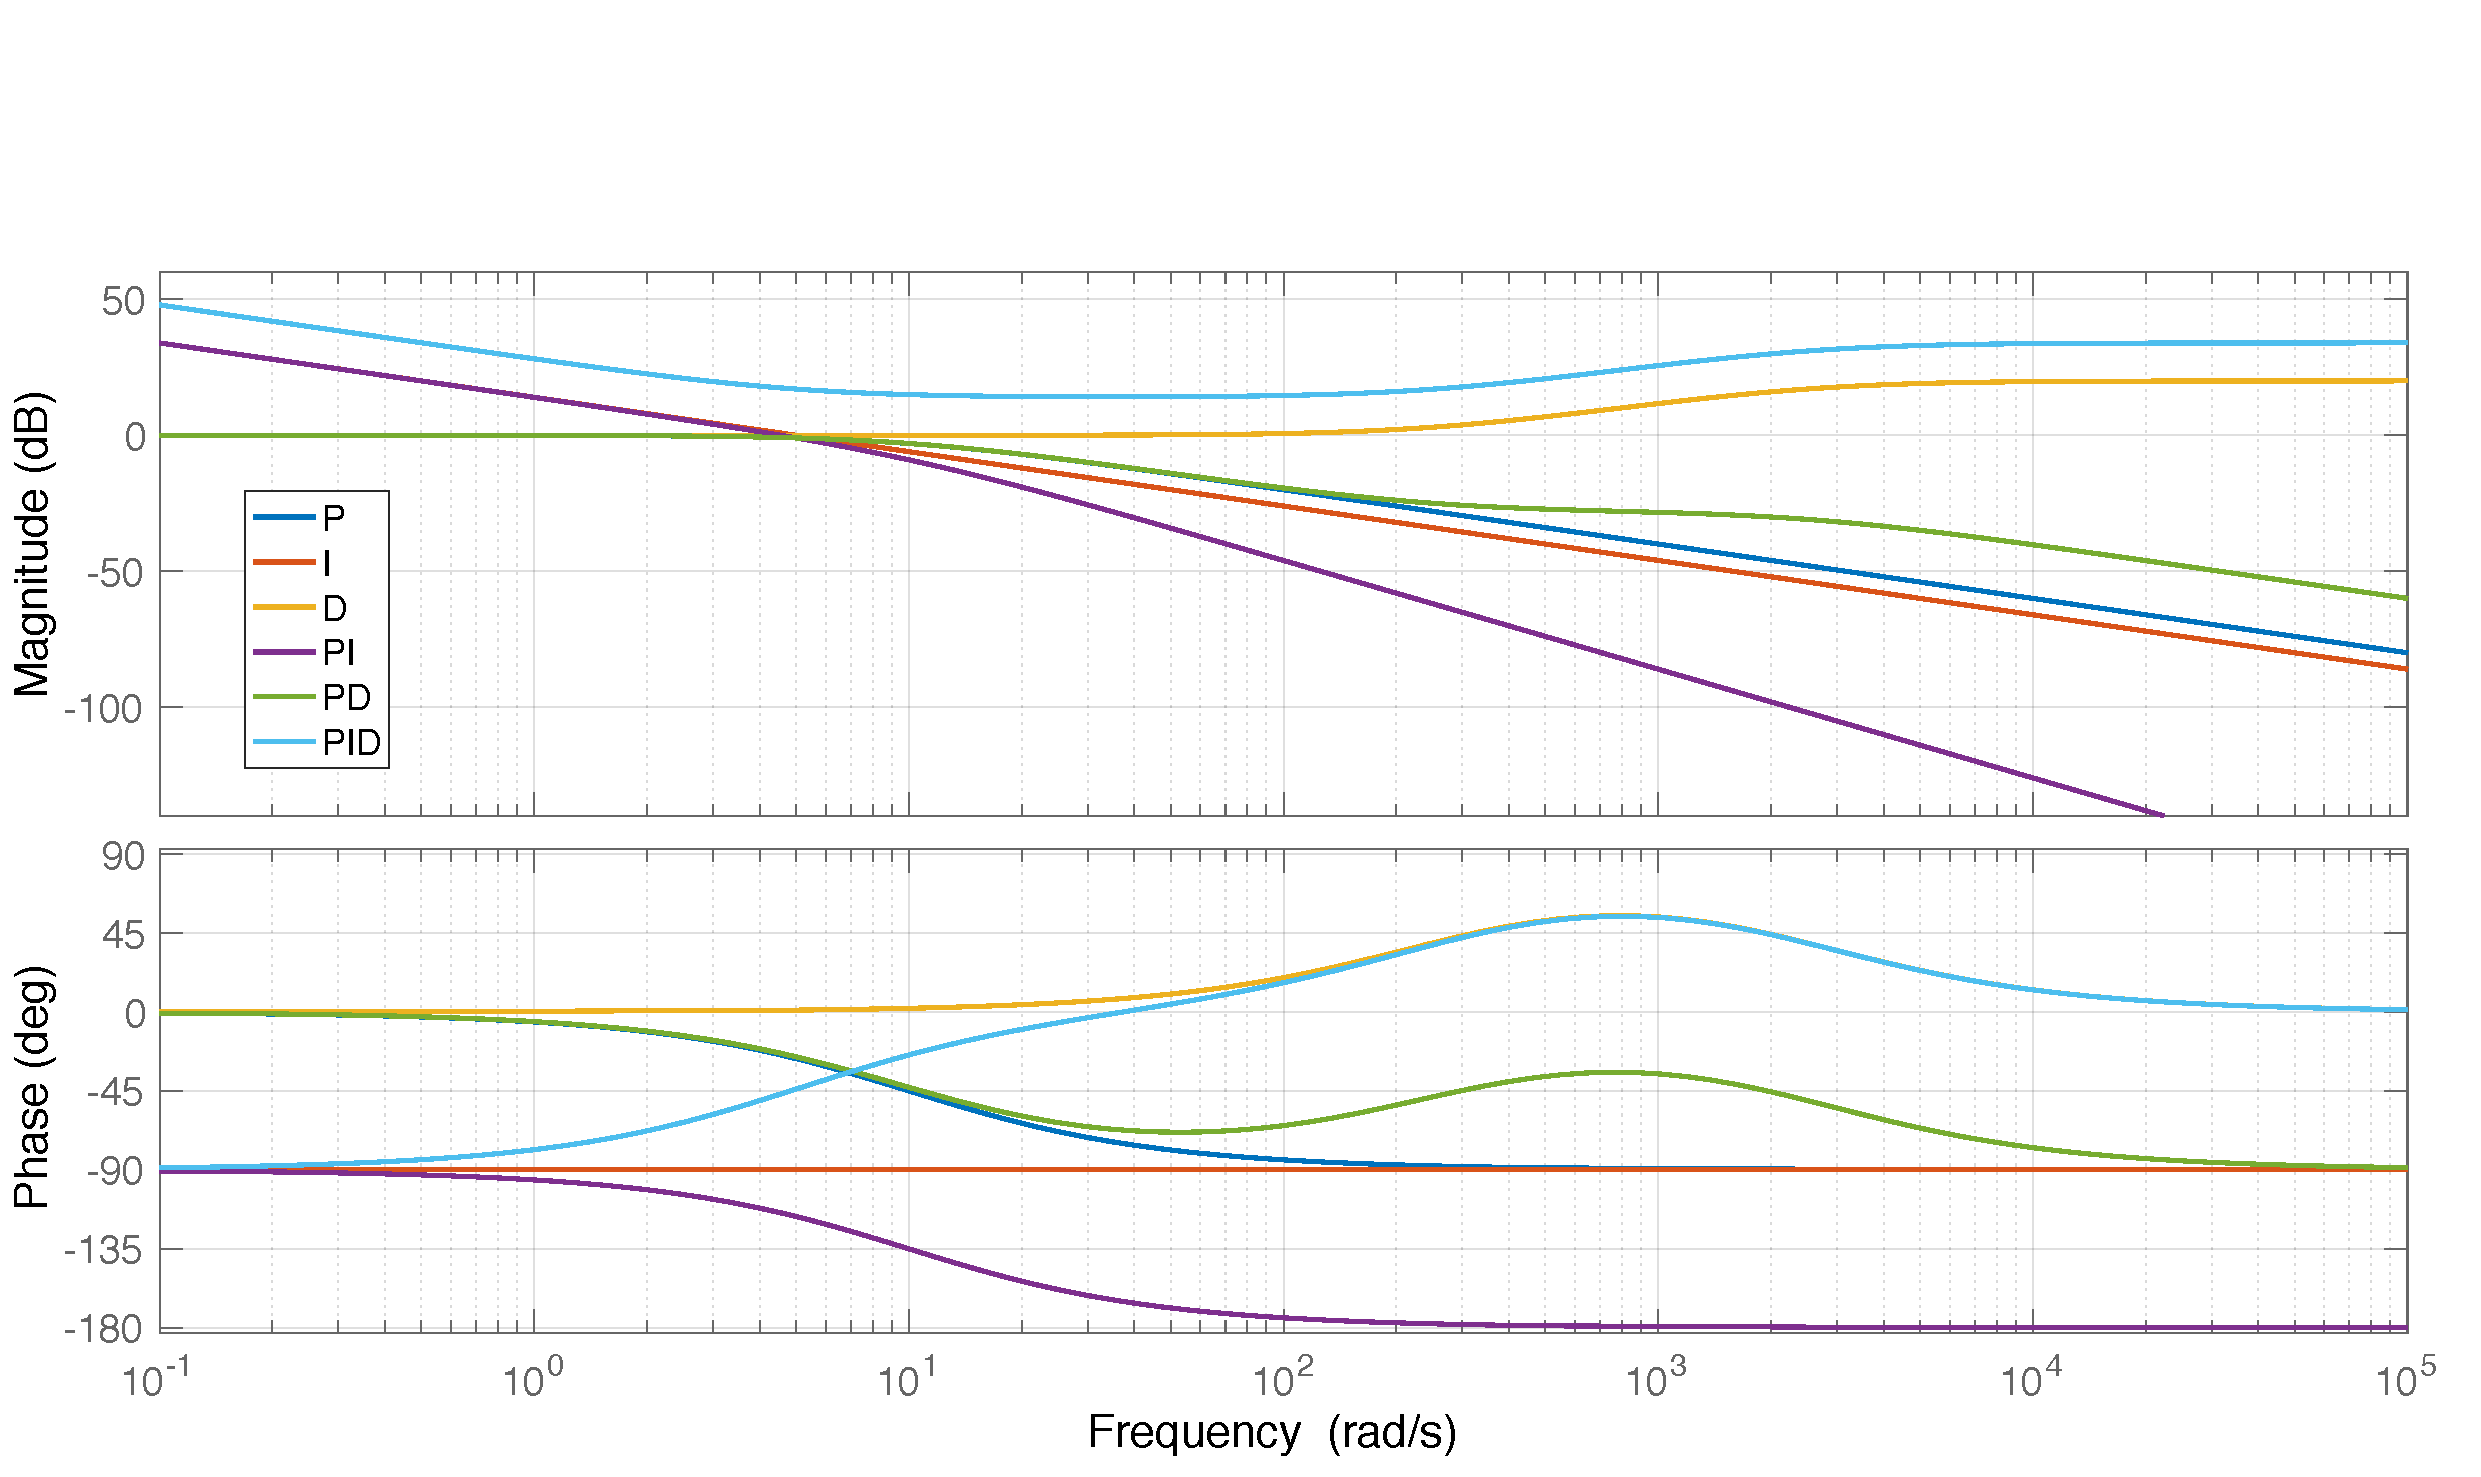
\includegraphics[width=\textwidth]{figures/ch_design/controller/Bodeplot_PID.pdf}
    \caption{An example of the different bode plot for the different PID-control part, to illustrate how they work on the gain and phase, both individual and combine with another.}
    \label{fig:PID_bode}
\end{figure}
From this figure it can be seen how the gain and phase is affected by the changes in the $K_p$, $k_I$ and $k_D$. It is also visible to see that the integral controller affects the gain but not the phase, only when it is combined with the proportional controller. 
It can also be seen that the derivative controller change the phase but not the gain as much. All these combinations can be used in different ways, but first for this project a proportional controller will be calculated, this will be done in the next section.

% http://blog.opticontrols.com/archives/344
\section{Design of proportional controller}\label{sec:design_controller}
As it has been decided to use a proportional controller to regulate the system, the proportional gain $K_p$ has to be found. 
When finding the value of $K_p$ the requirements from chapter \ref{ch:Req} have to be taken into consideration. 
The requirements that have to be taken into consideration are:
\begin{itemize}
    \item Overshoot of max 30\%
    \item Settling time of  max 10 seconds
    \item Steady state of $\pm$5\%
\end{itemize}
To find $K_p$ we have to start finding the damping factor. From the allowed overshoot the damping ratio $\zeta$ can be found with the equation \ref{eq:dampingRatio} \cite{nise2007control}.
\begin{equation}\label{eq:dampingRatio}
    \zeta = \frac{-\ln(overshoot/100)}{\sqrt{\pi^2+\ln^2(overshoot/100)}}
\end{equation}
With a overshoot of 30\% the damping ratio are found to be 0.358, and from this ratio the phase margin $\Phi_M$ can then be found with the use of the equation \ref{eq:phaseMargin} \cite{nise2007control}.
\begin{equation}\label{eq:phaseMargin}
    \Phi_M = \arctan\left(\frac{2\zeta}{\sqrt{-2\zeta^2+\sqrt{1+4\zeta^4}}}\right)
\end{equation}
The phase margin is calculated to 0.682 radian which are equal to $39.09\degree$. By making a bode plot of the open loop term ($G(s)H(s)$) from  the diagram in figure \ref{fig:controlDiagram} can the gain adjustment be fund.
In figure \ref{fig:des_bodeplot} can the bode blot of $G(s)H(s)$ be seen, where the gain margin, at the phase margin of $39.09\degree$, can be fund to be 39.7 dB.
\begin{figure}[h]
    \centering
    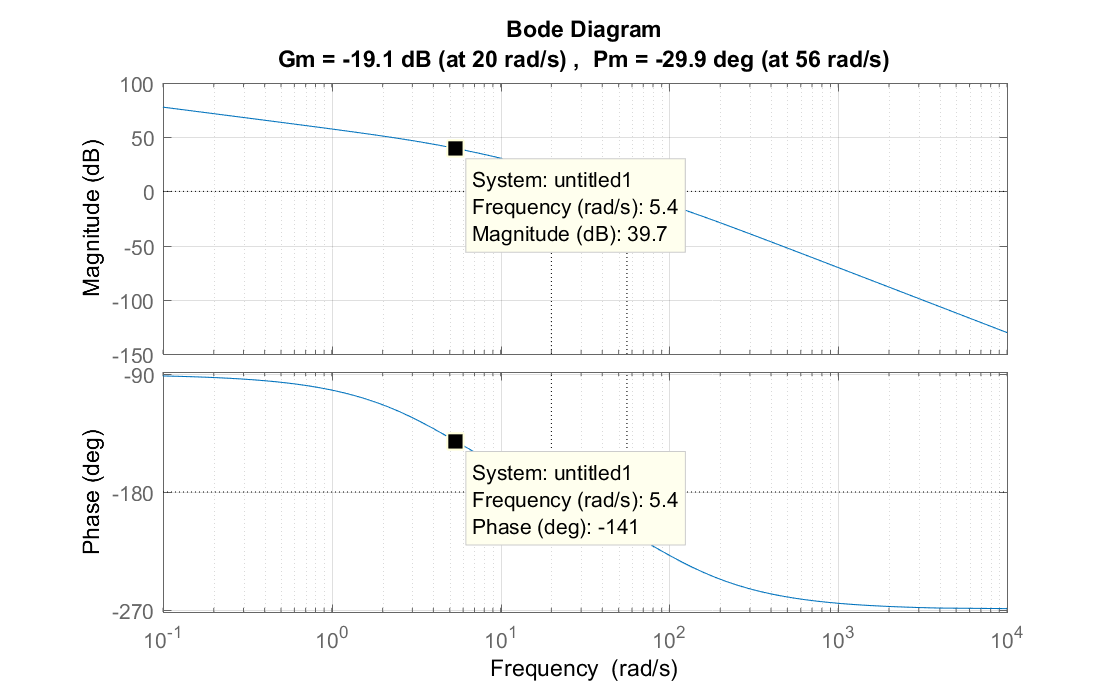
\includegraphics[width=0.8\textwidth]{figures/ch_design/controller/bodeplot.png}
    \caption{Bode plot of the open loop term ($G(s)H(s)$) with the phase margin of 39.09$\degree$ and the corresponding gain margin.} 
    \label{fig:des_bodeplot}
\end{figure}
\newline
To get the value of $K_p$ the magnitude have to be adjusted so the gain margin are 0 dB, this can be done by decreasing the calculated gain margin of 39.7 dB.
The -39.7 dB have to be converted to a gain factor, which have been done by using the following equation \(10^\frac{dB}{10}\) and calculated the factor to 0.01. This mean $K_p$ is 0.01.
With $K_p$ found the control diagram of the system get to be as seen in figure \ref{fig:dec_Final_block_diagram}.

\begin{figure}[H]
    \centering
    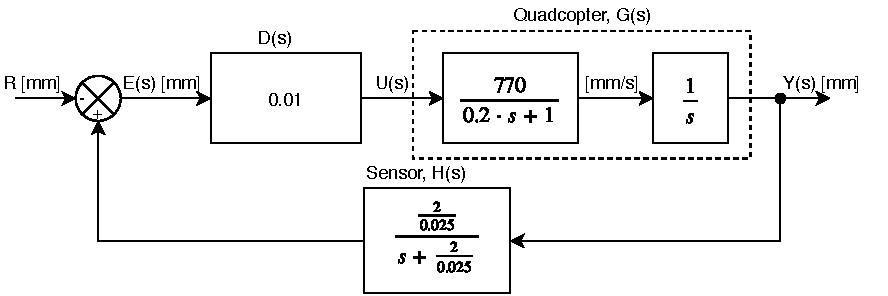
\includegraphics[width=\textwidth]{figures/ch_design/controller/FinalControlDiagram.pdf}
    \caption{Block diagram of the final control system.}
    \label{fig:dec_Final_block_diagram}
\end{figure}






